% =====================================================================
%  Mini-rapport — Semaine 1 (S1)
%  Projet 1 : Solveur de Nash m x n et duopoles (Cournot, Bertrand)
%  Groupe 1 — Théorie des Jeux et Systèmes Multi-Agents — ENSA Safi
%  Compilation : pdflatex S1_mini_rapport.tex   (2 passes)
% =====================================================================
\documentclass[11pt,a4paper]{article}

\usepackage[utf8]{inputenc}
\usepackage[T1]{fontenc}
\usepackage{lmodern}
\usepackage[french]{babel}
\usepackage{amsmath,amssymb}
\usepackage{geometry}
\usepackage{graphicx}
\usepackage{booktabs}
\usepackage{tabularx}
\usepackage{array}
\usepackage{enumitem}
\usepackage{microtype}
\usepackage{xcolor}
\usepackage{titlesec}
\usepackage{fancyhdr}
\usepackage{hyperref}

\geometry{margin=2.1cm}
\hypersetup{colorlinks=true, linkcolor=ensablue, urlcolor=ensablue}

% ---- Couleurs et style ----
\definecolor{ensablue}{RGB}{0,58,112}
\definecolor{ensagray}{RGB}{90,90,90}
\definecolor{okgreen}{RGB}{0,128,0}

\titleformat{\section}
  {\normalfont\large\bfseries\color{ensablue}}
  {\thesection.}{0.5em}{}
  [\vspace{-3pt}{\color{ensablue}\rule{\linewidth}{0.7pt}}]
\titlespacing*{\section}{0pt}{13pt}{6pt}

\setlist[itemize]{itemsep=2pt,topsep=3pt,parsep=0pt,leftmargin=1.3em}

% ---- En-tête / pied de page ----
\pagestyle{fancy}
\fancyhf{}
\fancyhead[L]{\small\color{ensagray}Projet 1 --- Groupe 1}
\fancyhead[R]{\small\color{ensagray}S1 --- Mini-rapport}
\fancyfoot[C]{\small\thepage}
\renewcommand{\headrulewidth}{0.4pt}
\renewcommand{\headrule}{\hbox to\headwidth{\color{ensablue}\leaders\hrule height \headrulewidth\hfill}}

\begin{document}

% ============================ PAGE DE GARDE ============================
\begin{titlepage}
\thispagestyle{empty}
\centering


\includegraphics[width=11cm]{logo_ensa.png}\par
\vspace{0.5cm}
{\color{ensablue}\rule{0.7\linewidth}{0.6pt}}\par

\vspace{1.8cm}

{\Huge\bfseries\color{ensablue} Mini-rapport --- Semaine 1 (S1)\par}

\vspace{0.7cm}
{\LARGE Cadrage et théorie\par}

\vspace{1.4cm}
{\large Projet 1 --- Solveur de Nash $m \times n$\\[2pt]
et duopoles (Cournot, Bertrand)\par}

\vspace{2.2cm}
{\large
Groupe 1 : ACHTOUK Fatine, ADIL Youness, BELHIMER Ikram, BOULHAIL Hiba\par
\vspace{0.5cm}
Module : Théorie des Jeux et Systèmes Multi-Agents --- ENSA Safi\par
\vspace{0.5cm}
Professeur : Abdelilah JRAIFI --- Année universitaire 2026-2027\par}

\vfill
{\large\bfseries 12 novembre 2026\par}
\vspace{0.4cm}
\end{titlepage}

% ============================ CORPS ============================
\section{Objectif de la semaine}

La semaine 1 est consacrée au \textbf{cadrage} du projet et à la \textbf{théorie} : poser les
fondations avant d'écrire le code. L'objectif est de disposer d'un dépôt, d'un environnement
de travail, d'une fiche de lecture théorique et d'un plan de travail (Gantt) validés par
l'équipe.

\begin{table}[h]
\centering
\caption{Bilan des attendus de la semaine 1}
\renewcommand{\arraystretch}{1.35}
\begin{tabularx}{\textwidth}{@{}p{4.7cm} >{\raggedright\arraybackslash}X c@{}}
\toprule
\textbf{Attendu (guide)} & \textbf{Réalisation} & \textbf{État} \\
\midrule
Dépôt GitHub créé
  & Dépôt du Groupe 1, branche \texttt{main}
  & \textcolor{okgreen}{\checkmark} \\
Ollama installé + \texttt{ollama pull llama3.1}
  & \texttt{llama3.1} (8B, \emph{tools}) + \texttt{llama3.2:3b}, serveur sur \texttt{127.0.0.1:11434}
  & \textcolor{okgreen}{\checkmark} \\
Fiche de lecture (Phase 0) rendue
  & \texttt{docs/fiche\_lecture.tex} $\rightarrow$ PDF
  & \textcolor{okgreen}{\checkmark} \\
Fonctions du cours à étendre identifiées
  & \texttt{nash\_mixte\_2x2} $\rightarrow$ \texttt{enumeration\_supports}, \texttt{est\_nash}, \texttt{cournot}, \texttt{cournot\_grille}
  & \textcolor{okgreen}{\checkmark} \\
Gantt prévisionnel déposé
  & \texttt{docs/gantt/} : Mermaid + CSV + PNG
  & \textcolor{okgreen}{\checkmark} \\
\bottomrule
\end{tabularx}
\end{table}

\section{Travail réalisé, par rôle}

Conformément à la règle n\textdegree~4, chaque membre a un rôle propre et au moins un commit
signé de son prénom.

\begin{itemize}
  \item \textbf{Théorie --- Fatine (chef de projet).} Formules de Nash, d'indifférence sur les
  supports, de Cournot et de Bertrand rédigées en LaTeX et expliquées « avec ses mots » ;
  hypothèses et limites listées ; conventions $A$/$B$ fixées avec les Groupes 2 et 6.
  \item \textbf{Quant / Python --- Ikram.} \texttt{src/jeux.py} : \texttt{est\_nash},
  \texttt{enumeration\_supports}, \texttt{cournot}, \texttt{cournot\_grille}, \texttt{bertrand}
  et les jeux de référence du cours (dilemme, bataille des sexes, pierre-feuille-ciseaux).
  \item \textbf{Développeur agent --- Youness.} \texttt{src/agent\_tj\_sma.py} : les deux
  nouveaux outils exposés au LLM, \texttt{resoudre\_bimatrice(A, B)} et
  \texttt{cournot(a, b, c, n\_firmes)}, avec plafonds et sortie JSON.
  \item \textbf{Testeur / Expérimentateur --- Hiba.} \texttt{tests/} : validation sur les trois
  jeux du cours, test hors ligne des outils (\texttt{.invoke}), ébauche de
  \texttt{src/experiences.py}.
\end{itemize}

\section{Rappels théoriques (formules clés)}

\paragraph{Équilibre de Nash.} Un profil $(x, y)$ est un équilibre de Nash si aucune déviation
\emph{pure} n'est profitable :
\[
(Ay)_i \le x^{\top} A y \quad \forall i, \qquad (x^{\top} B)_j \le x^{\top} B y \quad \forall j .
\]

\paragraph{Indifférence sur les supports.} Si $I$ (resp.\ $J$) est le support du joueur 1
(resp.\ 2), avec $|I| = |J| = k$, alors sur le support les gains purs sont égaux :
\[
(Ay)_i = v_1 \ \ (i \in I), \qquad (x^{\top} B)_j = v_2 \ \ (j \in J),
\]
d'où un système linéaire que l'on résout pour chaque couple de supports --- c'est le principe
de l'\textbf{énumération des supports}.

\paragraph{Cournot.} Avec $P(Q) = a - bQ$ et coût marginal $c$, la meilleure réponse est
$q_1 = (a - c - b\,q_2)/(2b)$ ; à l'équilibre symétrique à $n$ firmes,
\[
q^{*} = \frac{a - c}{(n+1)\,b}, \qquad \pi^{*} = \frac{(a-c)^2}{b\,(n+1)^2}.
\]
Pour le duopole de référence ($a = 100$, $b = 1$, $c = 10$) : $q^{*} = 30$, prix $40$,
profit $900$ par firme ; le cartel donnerait $q = 22{,}5$ et un profit $1012{,}5$.

\paragraph{Bertrand.} Concurrence en prix sur biens homogènes : l'équilibre est
$p_1 = p_2 = c$ et le profit est \textbf{nul} --- le \emph{paradoxe de Bertrand}.

\section{Livrables et vérifications}

\begin{itemize}
  \item \texttt{python -m pytest -q} : les tests passent (fonctions pures + outils sans LLM,
  aucun appel réseau).
  \item \texttt{python src/jeux.py} : affiche les équilibres des trois jeux du cours et
  Cournot ($q^{*} = 30$, profit $900$).
  \item \texttt{ollama list} : \texttt{llama3.1} (8B, \emph{tools}) disponible pour l'agent.
  \item \texttt{docs/fiche\_lecture.pdf} (Phase 0) et \texttt{docs/gantt/} (Gantt prévisionnel)
  déposés dans le dépôt.
\end{itemize}

\section{Difficultés rencontrées et solutions}

\begin{itemize}
  \item \textbf{Python 3.15 vs \texttt{zstandard}.} \texttt{langchain-core} $\rightarrow$
  \texttt{langsmith} $\rightarrow$ \texttt{zstandard}, qui n'a pas de wheel pour Python 3.15 ;
  \texttt{pip} tentait de le compiler et échouait (Visual C++ requis). \emph{Solution} :
  environnement dédié \texttt{.venv} sur \textbf{Python 3.12}, où tous les paquets s'installent
  en binaire (documenté dans \texttt{requirements.txt}).
  \item \textbf{Matrices passées en chaîne.} \texttt{llama3.1} envoie parfois
  $A = \texttt{"[[3, 0], [5, 1]]"}$ ; le validateur pydantic de LangChain rejetait la chaîne.
  \emph{Solution} : type \texttt{Matrice = Union[list, str]} dans \texttt{agent\_tj\_sma.py}
  (décodage \texttt{json.loads}, jamais \texttt{eval}), avec un test associé.
  \item \textbf{\texttt{ollama} absent du \texttt{PATH}.} Lancer l'application Ollama (serveur
  sur \texttt{127.0.0.1:11434}) ou appeler le chemin complet
  \texttt{\%LOCALAPPDATA\%\textbackslash Programs\textbackslash Ollama\textbackslash ollama.exe}.
\end{itemize}

\section{Écarts prévu / réalisé}

Aucun écart bloquant. L'installation de LangChain, initialement problématique, a été résolue
en travaillant sur Python 3.12 : l'agent LangChain réel est donc opérationnel \emph{dès S1},
soit une \textbf{avance} sur le planning prévisionnel (prévu en S3--S4). Le reste est
conforme au Gantt prévisionnel.

\section{Gantt prévisionnel}

\begin{figure}[h]
\centering
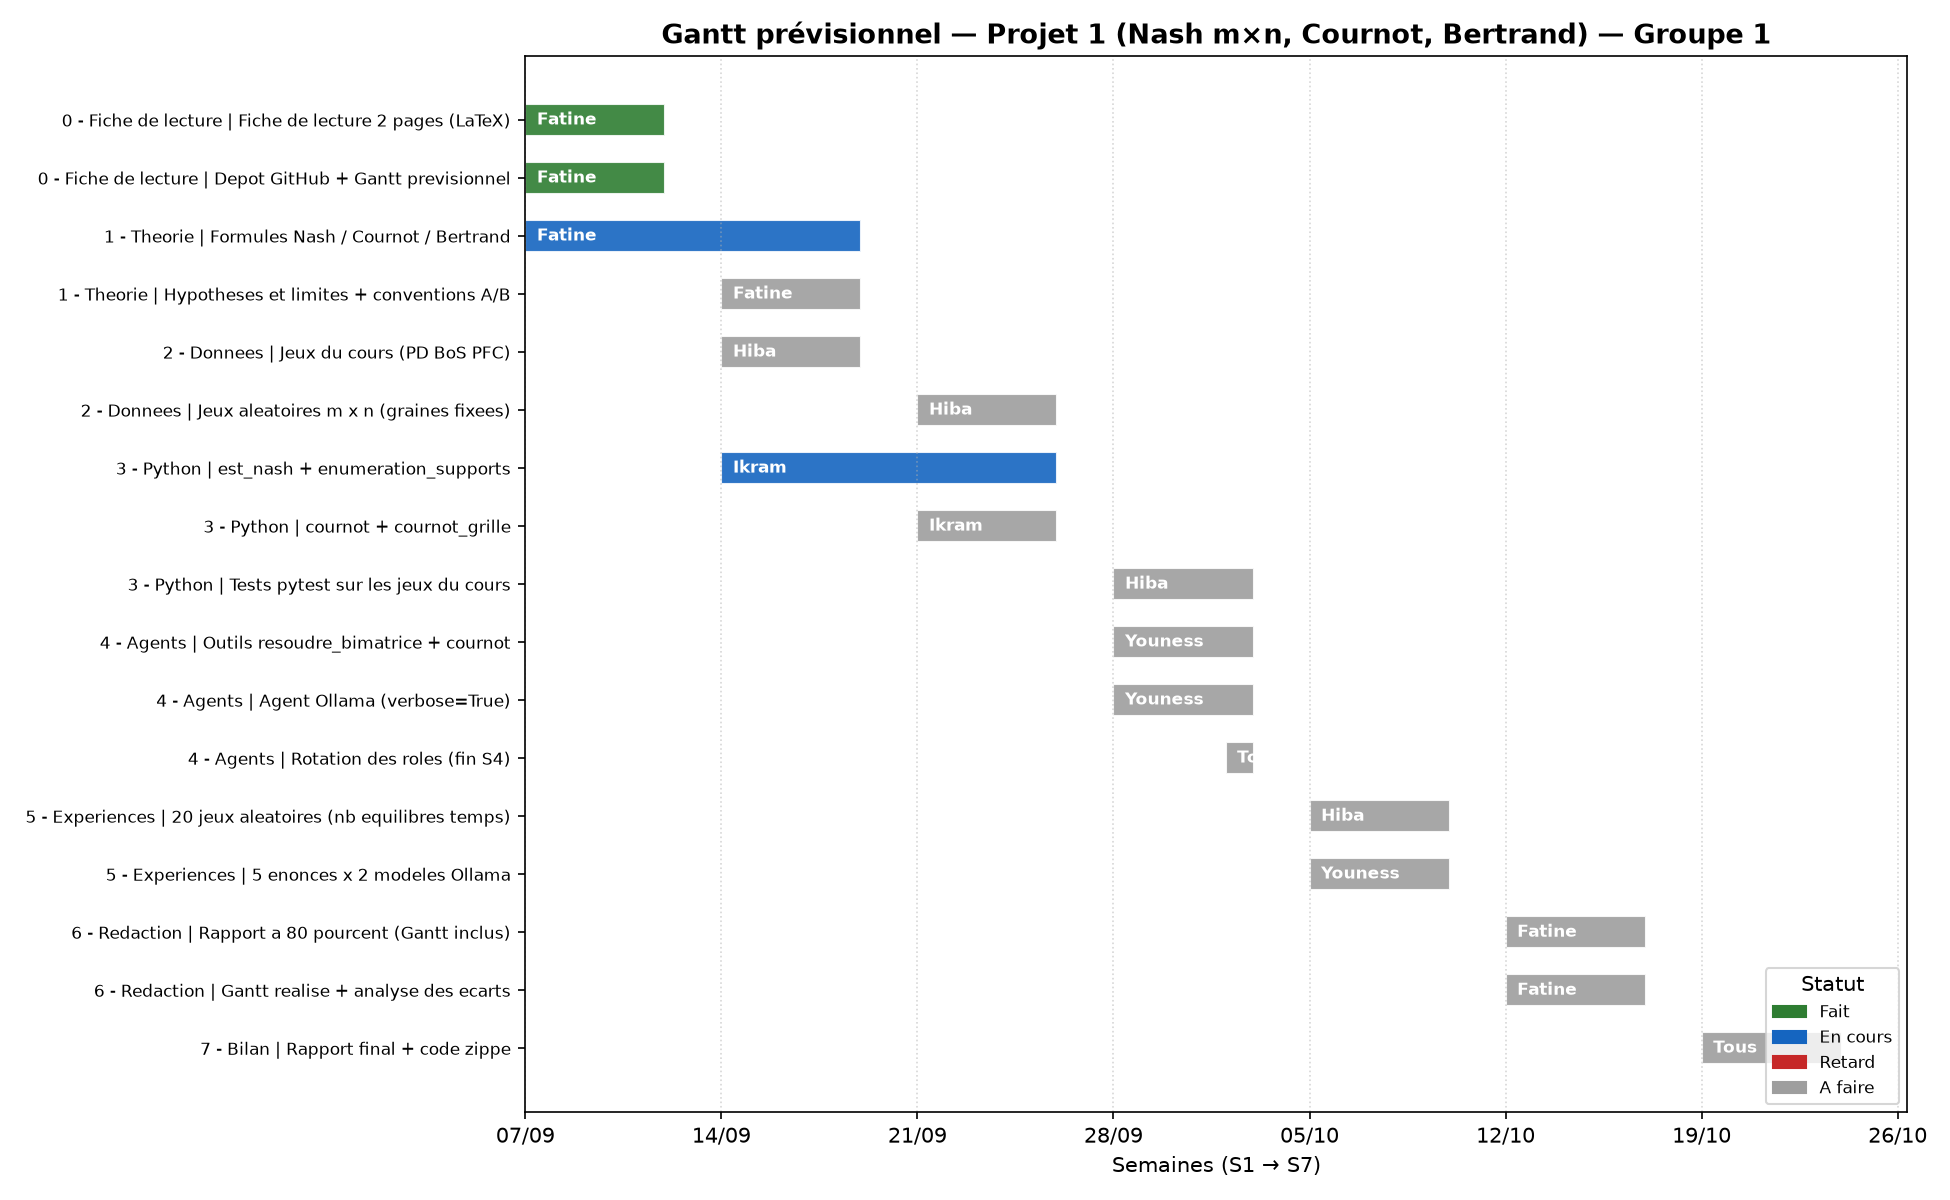
\includegraphics[width=0.98\textwidth]{gantt_previsionnel.png}
\caption{Gantt prévisionnel du projet (S1 $\rightarrow$ S7), avec la rotation des rôles
prévue en fin de S4.}
\end{figure}

\section{Plan de la semaine suivante (S2)}

\begin{itemize}
  \item Exécuter les fonctions dans \texttt{notebooks/01\_theorie\_prototype.ipynb} et
  reproduire les résultats du cours.
  \item Rédiger la section « formules expliquées » du rapport final.
  \item Lancer les 20 jeux aléatoires (\texttt{src/experiences.py}) et le banc d'essai
  \textbf{5 énoncés $\times$ 2 modèles} Ollama.
\end{itemize}

\section{État du dépôt Git (commits de la semaine)}

Chaque membre a poussé au moins un commit signé de son prénom entre crochets :
\begin{itemize}
  \item \texttt{[Fatine] Fiche de lecture Phase 0 (formules + hypothèses)}
  \item \texttt{[Ikram] Solveur de Nash m$\times$n : énumération des supports}
  \item \texttt{[Youness] Outils resoudre\_bimatrice et cournot exposés à l'agent}
  \item \texttt{[Hiba] Tests pytest des jeux du cours + tests hors ligne}
\end{itemize}

\end{document}
